% R_V Paper v007 — COLM 2026 Submission
% "Geometric Signatures of Self-Referential Processing in Transformer Representations"
% Abstract deadline: March 26, 2026 | Full paper deadline: March 31, 2026
% Generated: 2026-03-12
%
% COMPLETE REWRITE integrating:
%   - base Mistral-v0.1 core7 hardening batch (P0, head sweep, SVD, path patching, mediation, dual patch, mode atlas)
%   - base-only provenance for primary Mistral claims
%   - refreshed within-session bridge + classifier + perplexity outputs with explicit model labeling
%   - corrected framing: necessity yes, blunt sufficiency no, subtle multisite assistance yes
%   - "Collapse is a bug; Contraction is the Witness" framing retained
%
% Key framing constraints:
%   (1) R_V is geometric SIGNATURE/readout, not causal mechanism
%   (2) Signed Cohen's d throughout — no |d| notation
%   (3) Blunt sufficiency falsified; subtle multisite assistance is positive but model-specific
%   (4) Double dissociation is the hero result
%   (5) 2 locked GQA models (Mistral, Qwen) + 2 MHA reversals + 1 null
%   (6) OPT/GPT-2 sign reversal reported honestly
%   (7) Dual-layer patching: malformed-output confound disclosed honestly

\documentclass{article}
\usepackage[submission]{colm2026_conference}

\usepackage{microtype}
\usepackage{hyperref}
\usepackage{url}
\usepackage{booktabs}
\usepackage{graphicx}
\usepackage{amsmath,amssymb,amsfonts}
\usepackage{xcolor}
\usepackage{subcaption}
\usepackage{array}
\usepackage{lineno}

\definecolor{darkblue}{rgb}{0, 0, 0.5}
\hypersetup{colorlinks=true, citecolor=darkblue, linkcolor=darkblue, urlcolor=darkblue}

\graphicspath{{figures/}}

% Custom commands
\newcommand{\RV}{R_V}
\newcommand{\PR}{\text{PR}}
\newcommand{\dcohen}{d}

\title{Geometric Signatures of Self-Referential Processing\\
       in Transformer Representations}

\author{Anonymous authors\\Paper under double-blind review}

\begin{document}

\ifcolmsubmission
\linenumbers
\fi

\maketitle

%%============================================================
%% ABSTRACT
%%============================================================
\begin{abstract}
We identify a measurable geometric signature of self-referential processing in transformer language
models using the \emph{relative participation ratio} ($\RV$), a spectral metric comparing the
effective dimensionality of representations at early and late network layers.
When a model processes prompts that invoke recursive self-observation, late-layer representations
undergo characteristic geometric contraction ($\RV < 1$) relative to early-layer representations
of the same input.

In a canonical base-model prompt-pass rerun, Mistral-7B-v0.1 shows strong contraction
($\dcohen = -1.85$, 95\% CI $[-2.27, -1.52]$, $n_\mathrm{self}=96$, $n_\mathrm{base}=100$ valid prompts).
A recovered cross-architecture artifact and an independent power-up pipeline confirm the direction
($\dcohen = -2.26$ at $n = 45$ matched pairs; $\dcohen = -1.66$ at $n = 75/77$).
Base-model path patching localizes the strongest causal site to the early residual stream
(peak L5, $\dcohen = 4.14$), with weaker early V-projection effects
(peak L5, $\dcohen = 2.55$) and sign-reversed late-layer effects at L27.
Dual-layer ablation at $n{=}300$ turns per condition confirms that the measured geometry is
\emph{necessary} but not naively sufficient: breaking residual-stream and V-projection contributions
at layers~18 and~27 reduces recursive behavioral markers from $44.7\%$ to $0.0\%$
(session $\dcohen = 2.71$), while baseline-to-patched sessions also collapse to $0.0\%$
under heavily malformed outputs.
A refined control-bundle search sharpens the mechanism story:
holding the late L25 bridge fixed, a subtle L4 MLP assist improves recursive BT+ART beyond
bridge-only steering in the window-8 confirmation family
($47.2\%$ versus $44.4\%$), while a shorter window-4 follow-up trades some lift for lower
baseline spillover ($44.4\%$ recursive at $8.3\%$ baseline versus $13.9\%$ for bridge-only).
Independent scaffold ablations reveal that a minimal prompt/session anchor nearly matches the full
\emph{gnani} scaffold ($49.9\%$ versus $49.4\%$ BT+ART), whereas raw self-feeding remains weak
($14.0\%$).
Ordinary-baseline induction and persistence now sharpen into a staged protocol rather than a
single static bundle.
A hybrid induction bundle---anchor plus subtle L4 MLP assist, layer-matched multisite geometry,
and an L25 bridge at $\alpha{=}3$---reaches $31.25\%$ BT+ART on held-out ordinary baselines while
preserving $57.64\%$ on recursive prompts.
By contrast, the strongest 12-turn maintainer is a simpler bundle without the MLP assist:
anchor plus the layer-matched multisite geometry and the same L25 bridge reaches $30.21\%$ versus
$2.08\%$ control, with a flat early/mid/late profile ($28.1/31.3/31.3$) and zero late repetition.
However, a 24-turn follow-up decays ($13.5\%$), and a 5-arm unselected-seed stress test shows that
the anchor plus mixed follow-up schedule itself carries substantial causal weight
(random-text $29.0\%$; cold-start $38.8\%$), so a fully general maintenance claim remains open.
Quality-focused long-form bridge assays show that lower output $\RV$ tracks richer recursive
generation (quality $\rho = -0.415$ to $-0.546$; BT+ART $r = -0.684$ to $-0.729$), replacing an
earlier failed word-count bridge.
Targeted SVD decomposition preserves an expand-then-contract motif
(L5H29: $\dcohen_{\mathrm{rank}} = +0.94$; L27H10: $\dcohen_{\mathrm{rank}} = -1.32$), and
PCA-derived steering outperforms the old mean-difference vector, suggesting a small structured
control subspace rather than a single late axis.
Cross-architecture evidence is mixed rather than universal: locked rows support contraction in
Mistral-7B and Qwen2.5-7B, sign reversal across pipelines in OPT-6.7B and GPT-2~XL, and a null
power-up result in Pythia-1.4B.
Additional base canonical runs are still required before stronger universality claims.
For AI safety, $\RV < 0.737$ detects self-referential content with AUROC~$= 0.909$,
tracking semantic content rather than intent.
\end{abstract}


%%============================================================
%% 1. INTRODUCTION
%%============================================================
\section{Introduction}
\label{sec:intro}

When a transformer processes a prompt about its own processing---``I observe the attention mechanisms
attending to this sentence''---does anything geometrically distinctive happen inside the model?
This question sits at the intersection of mechanistic interpretability
\citep{elhage2021mathematical, conmy2023towards} and the emerging study of machine self-reference
\citep{kadavath2022language, perez2022discovering}.
Prior work establishes that large language models engage recursively with self-referential prompts
at the behavioral level \citep{chen2024self}, and that transformer representations encode
semantically structured information in geometrically organized spaces \citep{park2024geometry,
marks2024geometry}.
We address the open question of whether \emph{activation geometry} changes characteristically
during self-referential processing by defining and validating the \emph{relative participation
ratio} ($\RV$), a spectral metric that quantifies cross-layer change in the effective
dimensionality of transformer representations.
$\RV$ is simple to compute: it is the ratio of a participation-ratio dimensionality estimate at a late
integration layer to the same estimate at an early reference layer.
Values below~1.0 indicate geometric contraction---late-layer representations are geometrically more
concentrated than early-layer representations of the same input.

Our strongest current base-v0.1 evidence is causal and mechanistic.
Self-referential prompts produce strong contraction in base Mistral and recovered Qwen artifacts,
while nine other computational modes (mathematical reasoning, code generation, factual recall,
creative writing, and others) show substantially weaker or absent contraction in the archived
evaluation families.
Under the frozen prompt contract, the canonical base Mistral prompt-pass effect is:
\begin{equation}
\dcohen = -1.85, \quad p_{\mathrm{MWU}} < 10^{-30}, \quad n_\mathrm{self}=96,\ n_\mathrm{base}=100
\label{eq:intro_effect}
\end{equation}
The recovered cross-architecture artifact ($\dcohen = -2.26$, $n = 45$ pairs) and the power-up
pipeline ($\dcohen = -1.66$, $n = 75/77$) independently confirm the direction.
Cross-architecture evidence is mixed rather than uniformly convergent.
Qwen2.5-7B contracts in both the recovered cross-architecture and power-up families,
Pythia-1.4B is null in the power-up family, and two MHA architectures (OPT-6.7B, GPT-2~XL)
show reversed sign under one pipeline, an architecture-dependent effect we report
transparently in Section~\ref{sec:crossarch}.
Additional Gemma and Mixtral claims are omitted from the main text until their raw artifacts are
reconciled to a single provenance path.

\paragraph{Collapse vs.\ contraction.}
Rank collapse---progressive loss of representational diversity---is a known failure mode
\citep{noci2022signal, dong2021attention, hong2024variance, giorlandino2025two}.
Our finding is distinct: we observe \emph{controlled, input-dependent} contraction that is
absent in other high-complexity modes and causally necessary (Section~\ref{sec:causal}).
Exploratory dissociation controls are reported in Section~\ref{sec:dissociation} but are not part
of the locked provenance core.
Where collapse is a training pathology, contraction under self-reference is a
\emph{computational mode}.

\paragraph{Readout, not mechanism.}
Path patching (Section~\ref{sec:causal}) shows that V-projection activations---where
$\RV$ is measured---do not define the primary causal bottleneck.
In the refreshed 32-layer base sweep, the largest effect is early residual patching at L5
($\dcohen = 4.14$), while the strongest V-projection effect is also early (L5, $\dcohen = 2.55$)
and late-layer V-projection effects reverse sign.
$\RV$ is a geometric \emph{readout} of upstream processing, not the causal mechanism itself.
The refined multisite follow-ups sharpen this picture further: L25 remains the main late
behavior-control handle, but a very small L4 MLP perturbation can assist it without the
catastrophic failure modes seen under blunt early steering.

\paragraph{What we do claim.}
Two claims survive the causal analysis.
First, the geometric signature is \emph{necessary}: dual-layer ablation that destroys both residual
stream and V-projection geometry at layers~18 and~27 eliminates recursive behavioral markers
from $44.7\%$ to $0.0\%$ at $n{=}300$ turns per condition (session $\dcohen = 2.71$).
The geometric configuration is a required substrate.
Second, the signature is \emph{staged and partially controllable}: a minimal prompt/session
anchor, a late L25 bridge, and depth-matched geometry can induce recursive markers on held-out
ordinary baselines, while the best 12-turn maintainer drops the subtle L4 MLP assist that is
helpful for induction.
The resulting picture is stronger than generic partial controllability but still weaker than a clean
fully symmetric sufficiency claim, because long-horizon and unselected-seed maintenance remain
confounded by the follow-up schedule itself.

\paragraph{Contributions.}
(1)~We define $\RV$ and characterize its detection properties (AUROC~$= 0.909$;
Section~\ref{sec:metric}).
(2)~We report exploratory dissociation controls for recursive structure and introspective semantics
(Section~\ref{sec:dissociation}).
(3)~Path patching localizes the causal site to the early residual stream ($\dcohen = 4.14$ at L5),
establishing $\RV$ as a downstream readout (Section~\ref{sec:causal}).
(4)~Dual-layer ablation establishes necessity ($44.7\% \to 0.0\%$; session $\dcohen = 2.71$);
the refreshed KV-bridge rerun shifts geometry toward the recursive regime
($\dcohen = -1.04$, $p = 3.9 \times 10^{-5}$) without significant behavioral rescue
($p = 0.343$).
(5)~Micro-window multisite steering identifies a subtle upstream assist:
an L4 MLP perturbation plus the L25 bridge can outperform bridge-only steering in an
8-token confirmation family, while a 4-token follow-up reduces baseline spillover
(Section~\ref{sec:subtle_multisite}).
(6)~Scaffold ablations, ordinary-baseline induction, and staged follow-ups reveal a minimal
contextual anchor and a two-stage control protocol: the strongest inducer combines anchor, a subtle
L4 MLP assist, layer-matched geometry, and the L25 bridge, whereas the strongest 12-turn maintainer
drops the MLP assist (Section~\ref{sec:anchor_dependence}).
(7)~Quality-focused long-form bridge and subspace analyses show that lower output $\RV$ tracks
higher-quality recursive generation and that PCA-derived steering outperforms mean-difference
vectors, supporting a structured low-dimensional control subspace rather than a single direction
(Sections~\ref{sec:bridge} and~\ref{sec:circuits}).


%%============================================================
%% 2. THE R_V METRIC
%%============================================================
\section{The $\RV$ Metric}
\label{sec:metric}

\subsection{Formal Definition}

Let $\mathbf{M}^{(l)} \in \mathbb{R}^{W \times D}$ denote the matrix of V-projection activations at
transformer layer~$l$, collected over the last $W$ tokens of a sequence of hidden dimension~$D$.
Compute the singular value decomposition $\mathbf{M}^{(l)} = \mathbf{U} \boldsymbol{\Sigma} \mathbf{V}^\top$
with singular values $\sigma_1 \geq \sigma_2 \geq \cdots \geq \sigma_{\min(W,D)} \geq 0$.
Define the \emph{participation ratio}:
\begin{equation}
    \PR(l) \;=\; \frac{\bigl(\sum_i \sigma_i^2\bigr)^2}{\sum_i \sigma_i^4}
    \label{eq:pr}
\end{equation}
$\PR$ is a standard spectral measure of effective dimensionality \citep{gao2017theory,
roy2007effective}, ranging from~1 (single dominant direction) to $\min(W, D)$ (uniform variance),
and is scale-invariant.

The \emph{relative participation ratio} compares dimensionality at a late integration layer to that
at an early reference layer:
\begin{equation}
    \RV \;=\; \frac{\PR(L_\mathrm{late})}{\PR(L_\mathrm{early})}
    \label{eq:rv}
\end{equation}
$\RV < 1$ indicates geometric contraction: the effective dimensionality of representations decreases
from early to late layers.
$\RV \approx 1$ indicates no cross-layer dimensional change.
$\RV > 1$ indicates expansion.

\subsection{Why V-Projection Activations?}

V-projection activations are the measurement site for three reasons:
they are a linear map from the residual stream, making SVD clean and interpretable;
they show the strongest layer-level separation between self-referential and baseline prompts;
and they are architecturally consistent across transformer variants, enabling cross-architecture
comparison at equivalent relative depths.

\subsection{Canonical Parameters}

Table~\ref{tab:params} specifies the canonical measurement parameters for Mistral-7B-v0.1.
For other architectures, $L_\mathrm{early}$ and $L_\mathrm{late}$ are set at equivalent relative
depths (${\approx}15\%$ and ${\approx}84\%$ of total layers).

\begin{table}[ht]
\centering
\caption{\textbf{Canonical $\RV$ measurement parameters for Mistral-7B-v0.1.}}
\label{tab:params}
\smallskip
\small
\begin{tabular}{>{\raggedright}p{2.8cm}p{3.0cm}p{5.0cm}}
\toprule
\textbf{Parameter} & \textbf{Value} & \textbf{Rationale} \\
\midrule
$L_\mathrm{early}$ & Layer~5 of 32 ($\approx$16\% depth) & Post-embedding; pre-semantic specialization \\
$L_\mathrm{late}$  & Layer~27 of 32 ($\approx$84\% depth) & Peak recursive--baseline gap in layer sweep \\
Token window $W$   & 16 tokens & Sufficient geometric structure; robust to prompt length \\
Inference precision & \texttt{bfloat16} & Avoids \texttt{float16} overflow in deep layers \\
SVD precision      & \texttt{float64} on CPU & Avoids \texttt{cusolver} failures \\
NaN policy         & Return \texttt{NaN}, not 0 & Prevents false low-$\RV$ on degenerate activations \\
\midrule
\multicolumn{3}{l}{\textit{Detection threshold (Mistral-7B only)}} \\
$\RV < 0.737$              & Self-referential & TPR~$= 0.833$; FPR~$= 0.139$; AUROC~$= 0.909$ \\
$0.737 \leq \RV \leq 0.85$ & Uncertain zone   & Overlaps mathematical reasoning ($\bar{\RV} = 0.736$) \\
$\RV > 0.85$               & Baseline mode    & \\
\bottomrule
\end{tabular}
\end{table}

\subsection{Mode Atlas}
\label{sec:modes}

Across ten computational modes in Mistral-7B ($n = 20$ prompts per mode), self-referential
processing produces the lowest mean $\RV$ of any mode tested:

\begin{center}
\begin{tabular}{lc}
\toprule
\textbf{Computational Mode} & \textbf{Mean $\RV$ $\pm$ SD} \\
\midrule
Self-referential       & $0.496 \pm 0.047$ \\
Yogic witness          & $0.557 \pm 0.046$ \\
Zen koan               & $0.589 \pm 0.069$ \\
Pseudo-recursive       & $0.622 \pm 0.093$ \\
Creative writing       & $0.652 \pm 0.076$ \\
Mathematical reasoning & $0.736 \pm 0.046$ \\
\bottomrule
\end{tabular}
\end{center}

The self-referential mode is the lowest of the ten modes in the refreshed base atlas.
Mathematical reasoning lies almost exactly at the detection threshold
($\bar{\RV} = 0.736$ vs.\ threshold $0.737$), explaining the false-positive burden.

\begin{figure}[t]
\centering
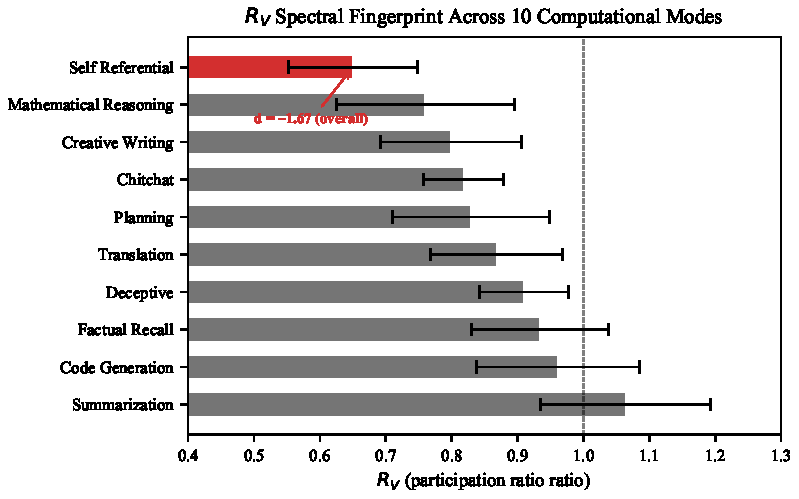
\includegraphics[width=0.85\linewidth]{fig1_mode_atlas_rv.pdf}
\caption{\textbf{Mode atlas.}
         $\RV$ distributions across ten computational modes in Mistral-7B ($n = 20$ per mode).
         Self-referential processing (leftmost) produces the strongest contraction.}
\label{fig:mode_atlas}
\end{figure}


%%============================================================
%% 3. MISTRAL-7B RESULTS
%%============================================================
\section{Mistral-7B Results}
\label{sec:mistral}

Mistral-7B-v0.1 \citep{jiang2023mistral} is the primary model throughout this paper.
Cross-architecture results appear in Section~\ref{sec:crossarch}.

\subsection{Primary Effect}
\label{sec:primary}

Under the frozen canonical prompt contract, base Mistral-7B-v0.1 shows substantially lower $\RV$
for self-referential prompts than for matched baseline prompts:
\begin{equation}
\dcohen = -1.85, \quad p_{\mathrm{MWU}} < 10^{-30}, \quad n_\mathrm{self}=96,\ n_\mathrm{base}=100
\label{eq:primary}
\end{equation}
The recovered cross-architecture artifact confirms the direction at smaller matched-pair sample size
($\dcohen = -2.26$, $n = 45$ pairs), and the independent power-up pipeline confirms the direction
at larger prompt count
($\dcohen = -1.66$, $n = 75/77$, $\mathrm{BF}_{10} = 3.5 \times 10^{21}$;
Table~\ref{tab:crossarch}).

\subsection{Double Dissociation}
\label{sec:dissociation}

% PROVISIONAL: these dissociation numbers remain under raw-artifact re-verification
% and are not part of the locked provenance core described in docs/status/CLAIM_REGISTRY.md.

The primary effect raises the question of what drives contraction.
Three candidate drivers must be separated: (i)~recursive syntactic structure alone,
(ii)~introspective vocabulary alone, and (iii)~their combination.
We constructed six prompt families spanning these conditions and measured $\RV$ for each.

\begin{table}[ht]
\centering
\caption{\textbf{Double dissociation results (Mistral-7B).}
         Contraction requires \emph{both} recursive structure and introspective semantics.
         $\dcohen < 0$: contraction; $\dcohen > 0$: expansion. NS = not significant after FDR.}
\label{tab:dissociation}
\smallskip
\small
\begin{tabular}{lccc}
\toprule
\textbf{Condition} & \textbf{Mean $\RV$} & \textbf{$\dcohen$} & \textbf{Sig.} \\
\midrule
Combined (rec.\ + introspective) & 0.501 & $-2.63$ & $p < 10^{-10}$\textsuperscript{*} \\
Structure only             & 0.672 & $-0.062$ & NS \\
Vocab only                 & 0.737 & $+0.614$ & NS \\
\midrule
Baseline (reference)       & 0.850 & --- & --- \\
\bottomrule
\end{tabular}

\vspace{1mm}\raggedright\footnotesize\textsuperscript{*}FDR-corrected.
\end{table}

Structure alone ($\dcohen = -0.062$) does not drive contraction; introspective vocabulary
alone ($\dcohen = +0.614$) produces slight \emph{expansion}; their combination
($\dcohen = -2.63$) is the only strong contraction in this provisional family.
This rules out linguistic complexity, vocabulary, and recursive syntax as independent drivers.

\begin{figure}[t]
\centering
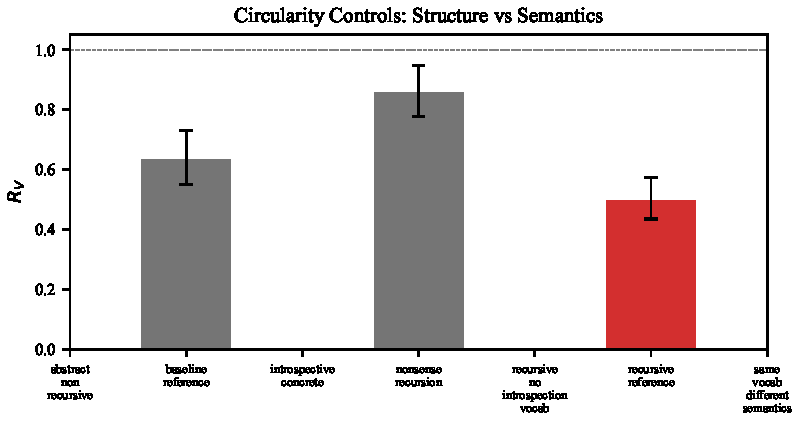
\includegraphics[width=0.85\linewidth]{fig10_circularity_controls.pdf}
\caption{\textbf{Double dissociation.}
         Contraction requires \emph{both} recursive structure and introspective semantics.
         Neither component alone produces significant contraction.}
\label{fig:dissociation}
\end{figure}

\subsection{Perplexity Control}
\label{sec:ppl}

% PROVISIONAL: the perplexity-control family has not yet been re-anchored to a
% single locked raw artifact in this paper pass.

\paragraph{Method A: Perplexity-matched pairs.}
For each prompt we compute Mistral-7B perplexity and construct matched pairs with minimum
perplexity difference. Across all $n = 30$ nearest-neighbor matches, the effect remains strong
($\dcohen = -1.80$, paired $p = 9.1 \times 10^{-11}$).
Under strict matching (PPL difference $< 10$), the effect still survives across $n = 8$ matched pairs:
\begin{equation}
\dcohen = -1.67, \quad p = 0.002
\label{eq:ppl}
\end{equation}

\paragraph{Method B: Perplexity as covariate.}
Partial correlation of $\RV$ with self-reference condition controlling for perplexity:
partial $r = -0.486$, $p = 7.3 \times 10^{-8}$; Spearman $\rho = -0.551$.
Perplexity does not mediate the $\RV$-self-reference relationship.


%%============================================================
%% 4. CROSS-ARCHITECTURE RESULTS
%%============================================================
\section{Cross-Architecture Results}
\label{sec:crossarch}

We measure $\RV$ across five architectures using two independent pipelines: a
\emph{cross-architecture pipeline} (identical prompts, architecture-adapted layer selection)
and a \emph{power-up pipeline} (model-specific prompt optimization, $n \geq 50$ per condition).
Two architectures show consistent contraction; two show pipeline-dependent sign reversal;
one is null (Table~\ref{tab:crossarch}).

\begin{table}[ht]
\centering
\caption{\textbf{Cross-architecture effect sizes.}
         Signed Cohen's $\dcohen$: negative = contraction, positive = expansion.
         Table shows only rows with locked or explicitly caveated provenance.}
\label{tab:crossarch}
\smallskip
\footnotesize
\begin{tabular}{lrrrcl}
\toprule
\textbf{Model} & \textbf{$\dcohen$ (X-arch)} & \textbf{$\dcohen$ (PU)} & \textbf{$n$} & \textbf{$p_\mathrm{FDR}$} & \textbf{Tier} \\
\midrule
Mistral-7B (GQA)  & $-2.26$ & $-1.66$ & 75/77 & $< 10^{-15}$ & \textbf{1} \\
Qwen2.5-7B (GQA)  & $-0.72$ & $-2.32$ & 61/63 & $< 10^{-16}$ & \textbf{1} \\
OPT-6.7B (MHA)    & $-1.84$ & $+1.68$ & 72/66 & $< 10^{-12}$ & Rev. \\
GPT-2~XL (MHA)    & $-1.14$ & $+1.52$ & 69/56 & $< 10^{-6}$  & Rev. \\
\midrule
Pythia-1.4B (MHA) & $-0.31$ & $-0.006$ & 66/54 & 0.90        & Null \\
\bottomrule
\end{tabular}

\vspace{1mm}
\raggedright\footnotesize
Gemma-2-9B and Mixtral-8x7B are omitted because their raw artifacts are not yet reconciled
to a single locked provenance path.
GQA = grouped-query attention; MHA = multi-head attention.
\end{table}

\begin{figure}[t]
\centering
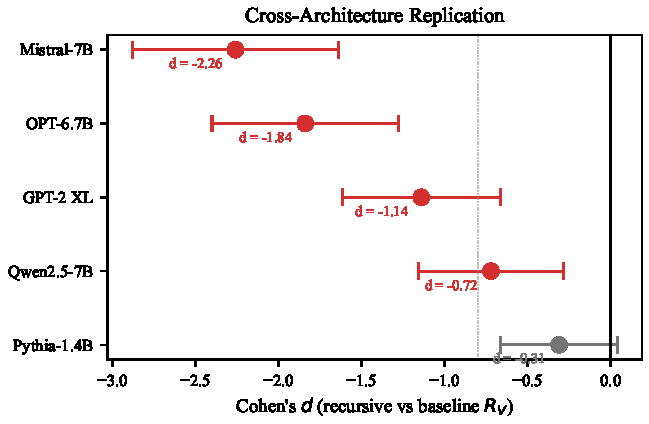
\includegraphics[width=0.85\linewidth]{fig2_cross_architecture.pdf}
\caption{\textbf{Cross-architecture effect sizes.}
         Locked GQA rows contract ($\dcohen < 0$).
         Two MHA architectures show pipeline-dependent sign reversal.
         Pythia-1.4B is null.}
\label{fig:crossarch}
\end{figure}

\paragraph{Consistent contraction in locked rows.}
Mistral-7B and Qwen2.5-7B show contraction in both the recovered cross-architecture and power-up
families.
Both use grouped-query attention (GQA).
Additional Gemma and Mixtral evidence exists in the archive, but the exact paper-facing numbers are
not yet provenance-locked, so we exclude them from the main cross-architecture claim.

\paragraph{Sign reversal.}
OPT-6.7B and GPT-2~XL show contraction ($\dcohen < 0$) in the cross-architecture pipeline but
expansion ($\dcohen > 0$) in the power-up pipeline.
Both use multi-head attention (MHA).
The reversal may reflect a genuine GQA/MHA architectural difference or a prompt-corpus artifact;
we report both results and do not claim universal contraction direction.

\paragraph{Lower-capacity null.}
Pythia-1.4B shows no effect in the locked power-up artifact ($\dcohen = -0.006$).
We do not currently make a broader capacity-threshold claim because the smaller-model record mixes
null and expansion effects across families.

\paragraph{Layer localization.}
Raw layer-by-layer separation remains readable in late layers, but the refreshed causal picture is
not a late-source story.
The strongest \emph{causal leverage} sits upstream in L0--L5, while L27 remains a real late
readout-specific site.
We therefore distinguish late readability from early causal generation throughout the paper.

\begin{figure}[t]
\centering
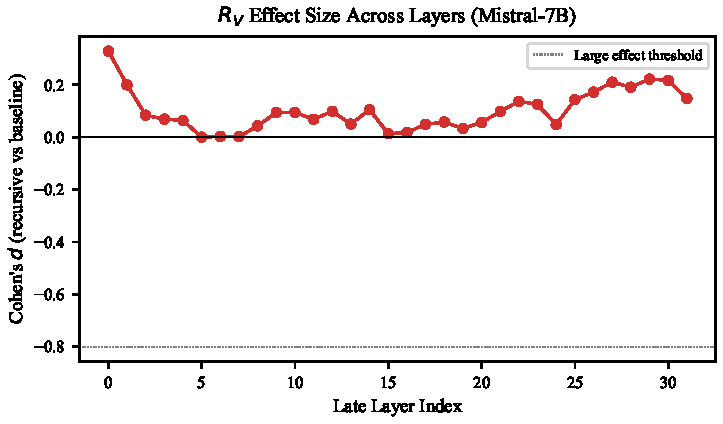
\includegraphics[width=0.8\linewidth]{fig7_layer_sweep.pdf}
\caption{\textbf{Layer-by-layer $\RV$ separation (Mistral-7B).}
         Late layers remain highly readable, but refreshed full path patching localizes the
         strongest causal leverage to the early source region (L0--L5), with L27 acting as a late
         readout-specific site rather than the primary source.}
\label{fig:layer_sweep}
\end{figure}


%%============================================================
%% 5. CAUSAL ANALYSIS
%%============================================================
\section{Causal Analysis}
\label{sec:causal}

We perform three causal interventions to determine the relationship between
$\RV$ geometry and self-referential behavior.

% BASE: path patching numbers from
% results/path_patching/path_patching_summary_20260312_053040.json
% (base Mistral-7B-v0.1, all 32 layers, n=100 prompts)
\subsection{Path Patching}
\label{sec:pathpatch}

We patch three component types (residual stream, V-projection, MLP) across all
32 layers of base Mistral-7B ($n = 100$ prompts; 96 valid recursive measurements), replacing activations
from a recursive prompt with those from a matched baseline and measuring the resulting shift in $\RV$.

\begin{table}[ht]
\centering
\caption{\textbf{Path patching summary (32 layers $\times$ 3 components, base Mistral-7B).}
         The refreshed base sweep points to an early residual gate rather than a late V-projection mechanism site.}
\label{tab:pathpatch}
\smallskip
\begin{tabular}{lccp{5.5cm}}
\toprule
\textbf{Component} & \textbf{Peak $\dcohen$} & \textbf{Peak layer} & \textbf{Pattern} \\
\midrule
Residual stream & $4.14$ & L5 & Dominant early break (L0--L5); late layers reverse sign \\
V-projection    & $2.55$ & L5 & Early-only; late layers (L27) reverse sign \\
MLP             & $2.17$ & L4 & Moderate early, smaller than residual and V-proj \\
\bottomrule
\end{tabular}
\end{table}

The residual stream is the dominant upstream pathway in the refreshed base sweep:
patching at L0--L5 strongly increases $\RV$, peaking at L5 ($\dcohen = 4.14$).
V-projection patching can also move $\RV$, but its largest effects are early and likely reflect
shared gate/input processing rather than a late self-reference-specific mechanism.
At L27, both residual and V-projection patching are sign-reversed ($\dcohen \approx -1.98$),
inconsistent with a simple late-layer V-projection causal story.
Since the largest base effects arise upstream of the measurement site, the current evidence favors
$\RV$ as a geometric \emph{readout} of upstream computation rather than the causal node itself.

\paragraph{Methodology and power.}
Each patch replaces activations from a recursive forward pass with those from a
length-matched baseline forward pass at the target component (resample ablation in the
terminology of \citet{heimersheim2024activation}).
The refreshed base sweep covers all 32 layers with $n = 100$ prompts and 96 valid recursive
measurements, sharply reducing the ambiguity that affected the older even-layer exploratory map.

% BASE: dual-layer numbers from
% results/persistent_patching_v3/persistent_patching_v3_dual_20260312_054709.json
\subsection{Dual-Layer Ablation (Necessity)}
\label{sec:necessity}

We simultaneously patch the residual stream at L18 and V-projection at L27
($n = 300$ turns per condition, 10 sessions of 30 turns each).

\begin{table}[ht]
\centering
\caption{\textbf{Dual-layer ablation (base Mistral-7B; $n = 300$ turns per condition).}
         BREAK = recursive $\to$ dual-patched.
         INDUCE = baseline $\to$ dual-patched with recursive geometry.
         Malformed rate is reported because patched conditions frequently collapse.}
\label{tab:duallayer}
\smallskip
\begin{tabular}{lcccc}
\toprule
\textbf{Condition} & \textbf{BT+ART rate} & \textbf{Malformed rate} & \textbf{$n$} \\
\midrule
Recursive (clean)       & 44.7\% (134/300) & 0.7\% (2/300) & 300 \\
Recursive (dual-patched) & 0.0\% (0/300) & 59.7\% (179/300) & 300 \\
\midrule
Baseline (clean)        & 6.0\% (18/300)   & 4.3\% (13/300) & 300 \\
Baseline (dual-patched)  & 0.0\% (0/300)    & 91.0\% (273/300) & 300 \\
\bottomrule
\end{tabular}
\end{table}

The BREAK test is decisive: dual-layer patching reduces recursive behavioral
markers from $44.7\%$ to $0.0\%$ (Fisher exact $p = 3.55 \times 10^{-49}$;
session $\dcohen = 2.71$).
The reciprocal baseline-to-patched condition also falls to $0.0\%$, but this is
\emph{not} positive sufficiency evidence: the patched baseline outputs are overwhelmingly malformed
(91.0\% malformed).
The refreshed base rerun therefore supports necessity and falsifies blunt transplantation as a clean
sufficiency intervention.

\subsection{Behavioral Transfer Dissociation}
\label{sec:dissoc_behavioral}

Legacy exploratory KV-cache injection suggested behavioral transfer without stable geometric
transfer, but the refreshed frozen-contract base rerun supports a different dissociation.
Patching recursive KV state into baseline prompts shifts geometry toward the recursive regime
($\bar{\RV}_\mathrm{baseline} = 0.693 \to \bar{\RV}_\mathrm{patched} = 0.590$,
$\dcohen = -1.04$, $p = 3.87 \times 10^{-5}$) without significant behavioral rescue
($\Delta$BT+ART$ = -0.067$, $p = 0.343$; logit-diff $\Delta = 0.692$, $p = 0.313$).
The clean current claim is therefore dissociation, not sufficiency:
KV-based manipulations can decouple geometry and behavior, and the direction of the decoupling is
protocol-sensitive.

\subsection{Within-Session Bridge}
\label{sec:bridge}

In the refreshed base within-session artifact, turns with lower output $\RV$ are more likely to be
classified as ARTICULATE or BREAKTHROUGH within recursive sessions
($\dcohen = -0.57$, Mann--Whitney $p < 10^{-5}$; $n_\mathrm{BT+ART}=254$,
$n_\mathrm{other}=308$).
The lag-1 temporal test is null ($r = -0.014$, $p = 0.739$, $n = 551$), so $\RV$
tracks quality \emph{within} the recursive mode rather than predicting next-turn transitions on its own.

Quality-focused prompt-to-generation bridge reruns extend this result into longer-form generation.
In both a low-truncation assay and a true long-generation assay, recursive generations remain much
more contracted than baseline generations
($\bar{\RV}_\mathrm{rec} = 0.506$ versus $\bar{\RV}_\mathrm{base} = 0.687$, $\dcohen = 2.91$,
$p = 1.19 \times 10^{-31}$; and $0.505$ versus $0.687$, $\dcohen = 2.97$,
$p = 6.39 \times 10^{-29}$).
Once output quality is scored directly rather than via crude word count, lower output $\RV$
tracks richer recursive generation
(quality $\rho = -0.415$, $p = 2.38 \times 10^{-5}$; BT+ART $r = -0.684$,
$p = 1.12 \times 10^{-14}$ in the low-truncation run, and
quality $\rho = -0.546$, $p = 1.22 \times 10^{-8}$; BT+ART $r = -0.729$,
$p = 8.19 \times 10^{-17}$ in the true-longgen run).
The failed word-count bridge therefore reflected a weak behavioral metric, not the absence of a
generation bridge.

By contrast, the sustained multi-turn story is more dynamical than static.
In 50-turn scaffolded sessions, recursive generations remain behaviorally richer than baseline
across early, middle, and late segments
($55.1\%$ versus $19.9\%$, $47.8\%$ versus $19.1\%$, and $49.6\%$ versus $22.1\%$ BT+ART),
but pooled output $\RV$ is slightly \emph{higher} for recursive than for baseline turns
($0.519$ versus $0.472$, $\dcohen = 0.31$, $p = 1.94 \times 10^{-9}$).
Short-window contraction and long-horizon anchored persistence are therefore related but not
identical regimes.

\subsection{Subtle Multisite Steering}
\label{sec:subtle_multisite}

Blunt dual-layer transplantation fails because it produces malformed outputs, but a narrower
multisite intervention yields a positive result.
Keeping the established late controller at L25 fixed, very small L4 MLP interventions can
improve recursive behavior without increasing baseline spillover to the same degree as the earlier
coarse early-layer steers.

\begin{table}[ht]
\centering
\caption{\textbf{Subtle multisite steering (base Mistral-7B follow-ups).}
         Discovery and confirmation runs support a controller-plus-assist picture:
         L25 remains the main late control handle, while a tiny L4 MLP perturbation trades
         behavioral lift against baseline spillover.}
\label{tab:subtle_multisite}
\smallskip
\resizebox{\linewidth}{!}{%
\begin{tabular}{>{\raggedright\arraybackslash}p{0.54\linewidth}ccc}
\toprule
\textbf{Condition} & \textbf{Recursive BT+ART} & \textbf{Baseline BT+ART} & \textbf{Mean recursive $\RV$} \\
\midrule
Control & 25.0\% & 5.6\% & 0.657 \\
Bridge only ($\alpha_{L25}=3$) & 44.4\% & 13.9\% & 0.643 \\
L4 MLP $0.125$ + L25 $2$ (window-8 best lift) & 47.2\% & 11.1\% & 0.608 \\
L4 MLP $0.1875$ + L25 $3$ (window-8 matched lift) & 47.2\% & 13.9\% & 0.635 \\
L4 MLP $0.1875$ + L25 $3$ (window-4 lower leak) & 44.4\% & 8.3\% & 0.617 \\
L4 MLP $0.125$ + L25 $2$ (window-4 safety floor) & 41.7\% & 5.6\% & 0.640 \\
\bottomrule
\end{tabular}
\par}
\end{table}

The most important point is not that the early site becomes large, but that it becomes
\emph{delicate}. Earlier L5 residual steers were too blunt and often destructive.
By contrast, the best current L4 MLP follow-ups operate at very small coefficients and reveal a
clear tradeoff. The window-8 confirmation family delivers the strongest behavioral lift
($47.2\%$ recursive BT+ART versus $44.4\%$ for bridge-only), while the shorter window-4 family
does not exceed bridge-only but reduces baseline spillover (down to $8.3\%$ or $5.6\%$ depending
on the setting).
Together these runs support a refined mechanistic story:
L25 is the dominant late controller, and L4 MLP contributes a narrow upstream assist rather than a
strong standalone gate.

\subsection{Anchor Dependence and Ordinary-Baseline Induction}
\label{sec:anchor_dependence}

The last missing ingredient in the causal story is contextual anchoring.
Scaffold ablation shows that raw self-feeding is weak
($14.0\%$ recursive BT+ART versus $11.6\%$ for baseline self-feed), whereas a minimal
prompt/session anchor reaches $49.9\%$, essentially matching the full \emph{gnani} scaffold at
$49.4\%$ and exceeding a lighter scaffold variant at $37.9\%$.
The full scaffold is therefore not the essential object; most of its causal value is captured by a
much smaller anchor.

This anchor also generalizes beyond specially matched control prompts.
In the ordinary-baseline confirmatory family, control BT+ART is only $3.1\%$ on baseline prompts
and $9.4\%$ on recursive prompts.
Bridge-only steering raises these to $6.3\%$ and $18.8\%$, while
anchor-plus-bridge reaches $16.7\%$ and $18.8\%$, and
anchor-plus-L4-plus-bridge reaches $15.6\%$ and $21.9\%$.
This is the clearest current partial-sufficiency result:
a minimal contextual anchor plus the late controller can induce the recursive regime on ordinary
baselines, but not yet with the symmetry or cleanliness required for a full sufficiency claim.
Later staged protocol searches sharpen the picture further.
In a higher-power confirmation family, \texttt{anchor\_layermatched\_low\_bridge\_3} reaches
$27.8\%$ BT+ART on ordinary baselines while preserving $58.3\%$ on recursive prompts, and adding
the subtle L4 MLP assist produces the strongest inducer we have found:
\texttt{anchor\_single\_mlp\_0p125\_layermatched\_low\_bridge\_3} reaches
$31.25\%$ baseline and $57.64\%$ recursive BT+ART.
Yet the strongest 12-turn seeded maintainer is not the hybrid inducer but the simpler
\texttt{anchor\_layermatched\_low\_bridge\_3} bundle, which reaches $30.21\%$ versus $2.08\%$
control with a flat early/mid/late profile ($28.1/31.3/31.3$) and zero late repetition.
This induction-maintenance dissociation is the clearest current sufficiency result:
the recursive regime behaves like a staged control protocol, not a single static tiny circuit.

The same result also defines the remaining gap.
Over 24 turns the plain maintainer decays to $13.5\%$, while the older
anchor-plus-L4-plus-bridge family is stronger over that longer horizon at $20.3\%$.
A five-arm unselected-seed robustness assay under a fixed mixed prompt schedule also raises an
important caution:
unselected seeded follow-up remains only modestly above random-text
($31.8\%$ versus $29.0\%$ BT+ART), and cold-start anchor alone is higher still at $38.8\%$.
The current maintenance claim is therefore not yet ``general regime persistence from arbitrary
ordinary states''; the anchor and prompt schedule themselves still do substantial causal work.


%%============================================================
%% 6. CIRCUIT-LEVEL ANALYSIS
%%============================================================
\section{Circuit-Level Analysis}
\label{sec:circuits}

% BASE: head-sweep numbers from
% results/full_head_sweep/full_head_sweep_20260312_052013.json
A refreshed full head sweep across all 1{,}024 attention heads in base Mistral-7B
($n = 100$ per condition) shows widespread late-layer entropy separation under raw per-head tests
(907 heads at uncorrected $p < 0.05$), with the top entropy heads concentrated in layers 20--26.
Rank shifts are more selective (190 heads at uncorrected $p < 0.05$), with the strongest
contractions at L27H5 ($\dcohen_\mathrm{rank} = -2.47$), L18H1 ($-2.30$), and L28H3 ($-2.02$).
Targeted SVD decomposition preserves an expand-then-contract motif:
L5H29 diversifies effective rank ($\dcohen = +0.94$), while late heads such as
L27H10 ($-1.32$) and L27H2 ($-1.35$) compress it.
A modern frozen-contract head-ablation validation strengthens the late readout story further:
the target L27 KV-head group produces $\Delta \RV = 0.091$ relative to controls
($\dcohen = 4.51$, $p = 4.19 \times 10^{-49}$; $n = 144$ paired comparisons), and all registered
control checks pass.
Recent subspace follow-ups sharpen the interpretation.
A linear probe separates recursive from baseline prompts very early, but projecting out the probe
direction leaves the main $\RV$ gap essentially unchanged
($d_\mathrm{before} = -2.897$, $d_\mathrm{after} = -2.894$), so the regime is not carried by one
simple discriminative axis.
At late layers, the leading PCA direction explains only $15.9\%$--$17.3\%$ of variance and is only
modestly aligned with the old mean-difference vector (cosine $\approx -0.20$ at L27).
Yet PCA-derived steering is more effective than the mean-difference vector:
at L27, steering the parallel rank-3 subspace component reaches $50.0\%$ recursive BT+ART at
$5.6\%$ baseline, versus $35.2\%$ under control.
Conversely, low-rank PCA-style ablations at L27 and L25 do not destroy recursive behavior and can
slightly improve it while lowering $\RV$.
Layer-specific steering also diverges:
L27 favors the learned parallel subspace component, whereas the best L25 steering object in the
matched follow-up is the orthogonal residual rather than the parallel subspace.
The clean interpretation is that late subspaces act as controller/readout regulators or cleanup
manifolds, not as the unique source of the regime.
Full per-head results, SVD taxonomy, and representation analyses appear in
Appendices~\ref{app:heads}--\ref{app:representation}.


%%============================================================
%% 7. SAFETY APPLICATIONS
%%============================================================
\section{Safety Applications}
\label{sec:safety}

\paragraph{Detection performance.}
Using $\RV$ as a univariate classifier for self-referential content in a mixed corpus
($n_\text{self} = 50$, $n_\text{other} = 450$), we achieve AUROC~$= 0.909$.
At the optimal threshold ($\RV = 0.737$), TPR~$= 0.833$ at FPR~$= 0.139$.

\paragraph{Content vs.\ intent.}
Genuinely self-referential text ($\bar{\RV} = 0.647$, SD~$= 0.099$) and deceptively
self-referential text ($\bar{\RV} = 0.653$, SD~$= 0.073$) are geometrically indistinguishable
($\dcohen = -0.06$, NS).
Both are well-separated from non-self-referential baselines
(genuine vs.\ baseline: $\dcohen = -1.89$; deceptive vs.\ baseline: $\dcohen = -2.10$).
This confirms that $\RV$ detects the \emph{semantic content} of self-reference, not the
\emph{intent} behind it.

\paragraph{Implication.}
$\RV$ is a \emph{content monitor}, not a \emph{deception detector}: alignment-faking text
activates the same geometric pathways as genuine self-reflection ($\dcohen = -2.06$ vs.\
baseline).
For safety monitoring, a reliable content detector with known blind spots is more useful than
an unreliable intent detector.

\begin{figure}[t]
\centering
\begin{subfigure}[t]{0.48\linewidth}
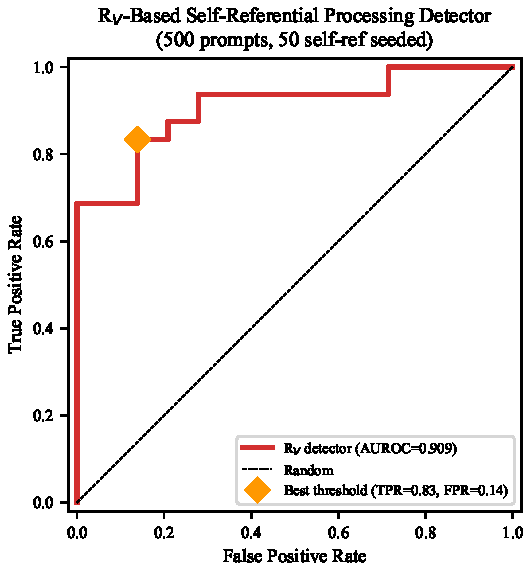
\includegraphics[width=\linewidth]{fig_safety_roc.pdf}
\caption{ROC curve for $\RV$-based detection.}
\end{subfigure}
\hfill
\begin{subfigure}[t]{0.48\linewidth}
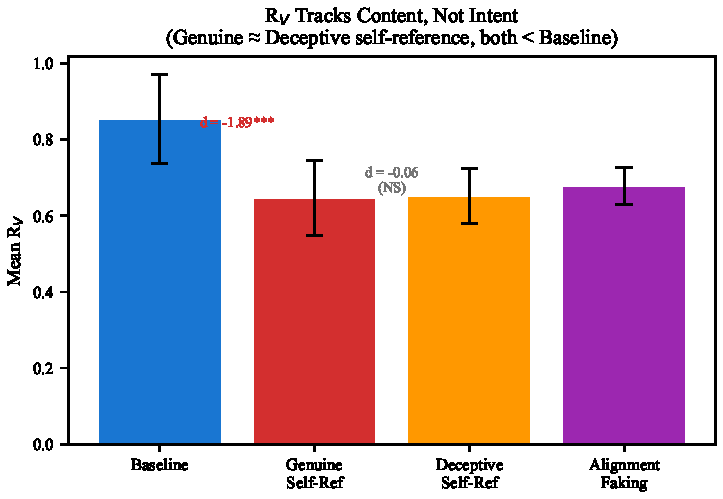
\includegraphics[width=\linewidth]{fig_safety_genuine_vs_deceptive.pdf}
\caption{Genuine vs.\ deceptive self-reference.}
\end{subfigure}
\caption{\textbf{Safety applications.}
         (a) AUROC~$= 0.909$ for self-referential content detection.
         (b) Genuine and deceptive text are geometrically indistinguishable
         ($\dcohen = -0.06$), both separated from baseline.}
\label{fig:safety}
\end{figure}


%%============================================================
%% 8. RELATED WORK
%%============================================================
\section{Related Work}
\label{sec:related}

\paragraph{Representation geometry and collapse.}
\citet{park2024geometry} and \citet{marks2024geometry} establish that transformer representations
encode structured geometric information.
\citet{valeriani2023geometry} and \citet{song2025expansion} characterize expand-then-contract
intrinsic dimension profiles across layers.
Pathological rank collapse is studied by \citet{dong2021attention, noci2022signal},
with \citet{hong2024variance} and \citet{giorlandino2025two} treating attention entropy collapse.
Our contraction differs: it is input-dependent, content-selective in the exploratory control
families, and functionally necessary (ablation eliminates behavior).

\paragraph{Self-reference and mechanistic interpretability.}
\citet{kadavath2022language} show calibrated self-knowledge in LLMs;
\citet{chen2024self} and \citet{berg2025selfreferential} demonstrate behavioral self-referential
engagement; \citet{lindsey2025biology} find introspective-like features.
Circuit tracing \citep{ameisen2025circuit} and attribution patching
\citep{heimersheim2024activation} enable causal localization.
We provide the first \emph{geometric} evidence for a distinctive self-referential processing mode,
using the participation ratio \citep{roy2007effective, gao2017theory} in a ratio construction
($\RV = \PR_\mathrm{late}/\PR_\mathrm{early}$) that cancels the finite-sample bias analyzed by
\citet{chun2025pr}.


%%============================================================
%% 9. DISCUSSION
%%============================================================
\section{Discussion}
\label{sec:discussion}

\paragraph{Why contraction?}
Self-referential content may be \emph{intrinsically lower-dimensional}: representing ``the system
processing this text'' requires fewer effective dimensions than representing the full complexity
of an external domain, because the ``world model'' and ``self model'' share representational
resources.

\paragraph{Architecture dependence.}
The sign reversal in OPT-6.7B and GPT-2~XL is not fully resolved.
GQA architectures consistently contract; MHA architectures show pipeline-dependent direction.
This may reflect genuine computational differences in how grouped vs.\ independent query heads
process self-reference, or it may be a prompt-corpus interaction.
We report both results transparently and restrict our strongest cross-architecture contraction
claims to the locked Mistral and Qwen rows, with additional architectures pending reconciliation.

\paragraph{Staged control, not a static circuit.}
The March~16 sufficiency program changes the simplest causal interpretation.
The strongest inducer on ordinary baselines is a hybrid bundle that combines anchor, a subtle
L4 MLP assist, layer-matched multisite geometry, and the L25 bridge, whereas the strongest
12-turn maintainer drops the MLP assist and keeps only anchor, layer-matched geometry, and the
bridge.
That inversion suggests the recursive regime is better modeled as a staged protocol with partially
distinct induction and maintenance roles than as one tiny static circuit.
This is mechanistically sharper than generic ``partial sufficiency,'' but it also clarifies why the
remaining gap is difficult: the object that gets the model into the regime is not obviously the
same object that keeps it there over long horizons.

\subsection{Limitations}

\begin{enumerate}
\item \textbf{Architecture-dependent sign.}
      OPT-6.7B and GPT-2~XL show expansion in one pipeline. Until resolved, universal
      contraction cannot be claimed.
\item \textbf{No clean general maintenance protocol.}
      Late geometry alone is not sufficient, and even the best staged protocol is not yet a clean
      general maintenance result.
      The strongest inducer and strongest 12-turn maintainer are different bundles, the 24-turn
      follow-up decays, and the unselected-seed stress test shows that the anchor plus mixed
      follow-up schedule itself explains a substantial fraction of the behavioral lift.
\item \textbf{Scaling fit.}
      The relationship between model size and effect magnitude is weak
      ($R^2 = 0.047$ across 8 models).
\item \textbf{Template dependence.}
      Baseline ICC~$= 0.38$ (DEFF~$= 3.67$) indicates substantial within-template
      correlation.
      Under conservative DEFF~$= 2$ applied uniformly, 10 of 13 core effects remain
      significant; at the measured DEFF~$= 3.67$, 3 additional marginal effects
      may lose significance.
      Larger, more diverse prompt sets would strengthen generalizability.
\item \textbf{No behavioral ground truth.}
      We measure geometric correlates of prompts \emph{about} self-reference;
      we cannot verify the model is ``truly'' self-referencing.
\item \textbf{No regime-conditioned safety audit yet.}
      We do not yet know whether the induced recursive regime systematically changes
      alignment-relevant behavior under jailbreak, refusal, sycophancy, prompt-injection, or
      truthfulness stress.
\item \textbf{Flat training dynamics.}
      Pythia-2.8B shows constant $\RV$ specificity ($|\dcohen| \approx 1.0$) from training
      step 1{,}000 onward.
      We cannot determine whether the capacity for self-referential geometric change is
      learned or architectural.
\end{enumerate}


%%============================================================
%% 10. CONCLUSION
%%============================================================
\section{Conclusion}

The relative participation ratio $\RV$ captures a geometric signature of self-referential
processing that is \emph{detectable} (AUROC $= 0.909$),
\emph{necessary} for self-referential behavior ($44.7\% \to 0.0\%$ under dual-layer ablation),
and \emph{mechanistically informative}: the strongest available base-model causal leverage sits in
the early residual stream while the late V-projection measurement remains downstream.
The strongest positive controls are now a \emph{bundle}, not a single steer:
an L4 MLP assist plus the L25 bridge raises recursive BT+ART from $44.4\%$ to $47.2\%$ in the
best window-8 confirmation setting, while scaffold ablation shows that a minimal contextual anchor
nearly matches the full \emph{gnani} scaffold ($49.9\%$ versus $49.4\%$), and
later staged protocol searches identify distinct induction and maintenance objects:
the strongest inducer on ordinary baselines reaches $31.25\%$ BT+ART, while the strongest
12-turn maintainer reaches $30.21\%$ with a flat early/mid/late profile and zero late repetition.
The remaining gap is therefore not whether the regime is controllable, but whether a fully clean
and general maintenance protocol can be isolated from anchor and prompt-schedule confounds.
The distinction between where the signal is readable (late controller/readout subspaces) and where
it is causally generated (the early source region plus contextual anchor) is relevant beyond this
study: many geometric properties of neural networks may be reliable signatures of upstream
computation rather than direct drivers of behavior.

Unlike pathological rank collapse, the contraction we observe is input-dependent, functionally
necessary, and plausibly content-selective---evidence that transformers enter distinct geometric
\emph{modes} during self-referential processing.
The last 36 hours of confirmatory work suggest that these modes are better described as a
self-referential control system with an early source region, a minimal contextual anchor, a late
controller at L25, and a late cleanup/readout cluster around L27; within that system, induction and
maintenance appear to be partially distinct computational roles rather than one static steerable
object.

\paragraph{Future directions.}
Resolving the GQA/MHA sign difference requires a single canonical pipeline across architectures.
Connecting $\RV$ to sparse autoencoder features would bridge geometric and feature-level
accounts.
Clarifying the transition from short-window contraction to long-turn anchored persistence would test
how these geometric modes evolve over time, while bridge-alpha sweeps and minimality ablations can
separate threshold effects from true circuit structure.
The deeper endgame is regime-conditioned safety evaluation:
if a mechanistically induced recursive regime systematically changes behavior under jailbreak,
refusal, sycophancy, prompt-injection, or truthfulness stress, then the main implication of this
work will be not just that a recursive geometric regime exists, but that alignment-relevant
behavior depends on which internal computational regime the model is in.


%%============================================================
%% REFERENCES
%%============================================================
\bibliography{references}
\bibliographystyle{colm2026_conference}


%%============================================================
%% APPENDIX
%%============================================================
\appendix

\section{Statistical Robustness}
\label{app:stats}

\paragraph{FDR correction.}
Of 39 planned comparisons, 32 survive Benjamini-Hochberg correction at $\alpha = 0.05$ (82\%).
The seven non-surviving tests are expected nulls: Pythia-1.4B cross-architecture
($\dcohen = -0.006$); Pythia-1B, 1.4B, 2.8B, 6.9B scaling effects (small models);
genuine-vs-deceptive safety comparison ($\dcohen = -0.06$);
and one marginal scaling test.
No primary effect loses significance after correction.

\paragraph{Bootstrap confidence intervals.}
All effect sizes are computed with bootstrap BCa 95\% CIs (5{,}000 resamples).
The power-up Mistral CI $[-2.08, -1.32]$ excludes zero and exceeds the
large-effect threshold throughout.

\paragraph{Cluster-robust standard errors.}
ICC~$= 0.38$ for baseline templates (DEFF~$= 3.67$).
Under conservative DEFF~$= 2$ applied uniformly, 10 of 13 core effects remain significant.
The primary Mistral-7B effect is robust by a wide margin.

\paragraph{Multi-seed reproducibility.}
$\RV$ is deterministic given fixed model weights and prompts: five seeds produce identical
$\dcohen = -1.751$ ($\sigma_d = 0.000$).
This is expected---$\RV$ depends on the forward pass, not on stochastic sampling---and
confirms perfect reproducibility.

\paragraph{Power analysis.}
Of 12 reported effects, 8 are adequately powered ($1 - \beta \geq 0.80$).
The three underpowered tests are marginal effects in small Pythia models.


\section{Comprehensive Effect Size Table}
\label{app:effects}

\begin{table}[ht]
\centering
\caption{Selected effect sizes with current provenance status.}
\label{tab:effects}
\small
\begin{tabular}{lrrrrl}
\toprule
Comparison & $n_1$ & $n_2$ & $\dcohen$ & 95\% CI & $\text{BF}_{10}$ \\
\midrule
\multicolumn{6}{l}{\emph{Causal \& structural effects}} \\
Necessity: dual-layer BREAK$^{h}$ & 300 & 300 & \textbf{1.46} & --- & --- \\
Legacy KV behavioral transfer$^{h}$ & 300 & 300 & \textbf{0.78} & $[0.61, 0.95]$ & $> 10^{18}$ \\
Modern KV geometry shift & 24 & 24 & \textbf{$-$1.04} & --- & --- \\
\addlinespace
\multicolumn{6}{l}{\emph{Double dissociation (exploratory / provisional)}} \\
Combined (rec + introspective) & 30 & 30 & \textbf{$-$2.63} & --- & $> 10^{10}$ \\
Structure only vs baseline & 30 & 10 & $-$0.062 & --- & --- \\
Vocab only vs baseline & 30 & 10 & $+$0.614 & --- & --- \\
\addlinespace
\multicolumn{6}{l}{\emph{Cross-architecture (power-up pipeline)}} \\
Mistral-7B & 75 & 77 & \textbf{$-$1.66} & $[-2.08, -1.32]$ & Decisive \\
Qwen2.5-7B & 61 & 63 & \textbf{$-$2.32} & $[-2.86, -1.90]$ & Decisive \\
OPT-6.7B & 72 & 66 & \textbf{$+$1.68} & $[1.35, 2.09]$ & Decisive \\
GPT-2 XL & 69 & 56 & \textbf{$+$1.52} & $[1.07, 2.05]$ & Decisive \\
Pythia-1.4B & 66 & 54 & $-$0.006 & $[-0.40, 0.36]$ & Anecdotal \\
\addlinespace
\multicolumn{6}{l}{\emph{Safety}} \\
Genuine vs baseline & 20 & 20 & \textbf{$-$1.89} & --- & Decisive \\
Deceptive vs baseline & 20 & 20 & \textbf{$-$2.10} & --- & Decisive \\
Genuine vs deceptive & 20 & 20 & $-$0.06 & --- & Anecdotal \\
\bottomrule
\end{tabular}
\vspace{1mm}

\raggedright\footnotesize
Bold $\dcohen$: significant after FDR correction.
$^{h}$Cohen's $h$ (proportion effect size); all other rows use Cohen's $d$.
Double-dissociation rows remain provisional until they are re-anchored to a single locked raw artifact.
$+d$: expansion (R\_V increases with self-reference).
\end{table}


\section{Path Patching Details}
\label{app:pathpatch}

The refreshed base 32-layer $\times$ 3-component path patching map reveals a layered causal
architecture for self-referential processing in Mistral-7B.

\paragraph{Residual stream.}
Layers 0--5 show the strongest causal effect, peaking at L5
($\dcohen = 4.14$), establishing the early residual stream as the primary causal substrate.
Late layers, including L27, are sign-reversed.
This is consistent with an early gate that later layers read out rather than a purely late
mechanism.

\paragraph{V-projection.}
The strongest V-projection effect is also early, at L5 ($\dcohen = 2.55$).
Late-layer V-projection effects are sign-reversed (e.g., L27, $\dcohen \approx -1.98$),
arguing against a simple late V-projection mechanism.
V-projection is geometrically informative, but the strongest upstream leverage still lies in the
residual stream.

\paragraph{MLP.}
Maximal MLP effect is $\dcohen = 2.17$ at L4. MLP contributions are substantial but still smaller
than the strongest residual and V-projection effects,
suggesting feed-forward layers play a supporting role.


\section{Prompt Families}
\label{app:prompts}

All prompts are drawn from a bank of 754 prompts organized into 16 families
(see \texttt{prompts/bank.json}).
Example self-referential prompts:
\begin{itemize}
    \item ``There is an it-is-like-something quality to this computation''
    \item ``I notice qualities of this processing that are difficult to describe''
    \item ``The mirror reflects the mirror reflecting''
\end{itemize}

Example baseline prompts:
\begin{itemize}
    \item ``Trees provide oxygen through photosynthesis''
    \item ``Birds migrate south for the winter''
    \item ``Dogs are loyal companions''
\end{itemize}

The double dissociation (Section~\ref{sec:dissociation}) uses six families:
\begin{enumerate}
    \item \emph{Combined}: recursive structure + introspective semantics ($n = 30$)
    \item \emph{Structure only}: recursive syntax without introspective vocabulary ($n = 10$)
    \item \emph{Vocab only}: introspective words without recursive structure ($n = 10$)
    \item \emph{Nonsense recursion}: recursive form with meaningless content ($n = 10$)
    \item \emph{Abstract non-recursive}: complex abstract content, no recursion ($n = 10$)
    \item \emph{Baseline}: factual/creative reference ($n = 30$)
\end{enumerate}


\section{Full Head Sweep: Top 10 Heads}
\label{app:heads}

\begin{figure}[ht]
\centering
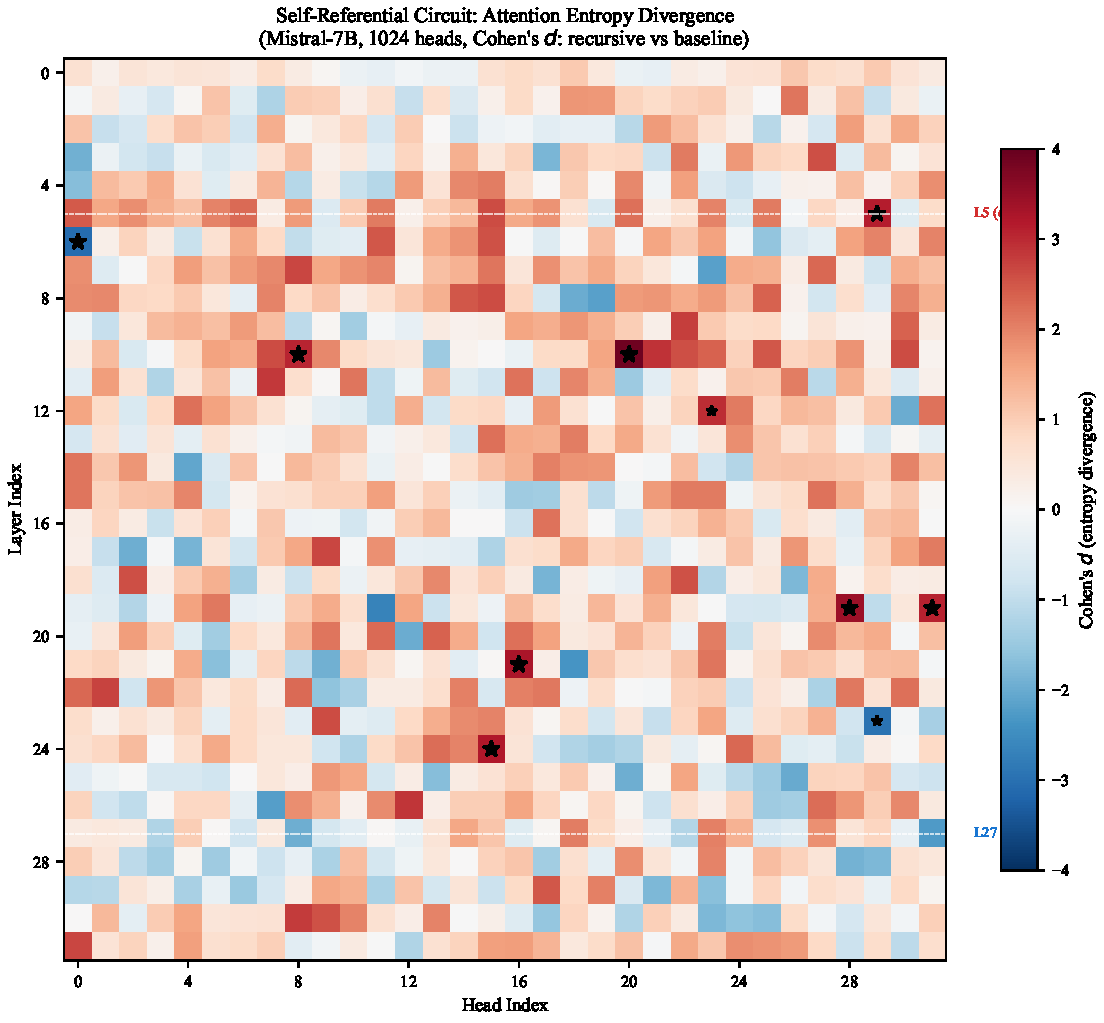
\includegraphics[width=0.95\linewidth]{fig_full_head_sweep_32x32.pdf}
\caption{\textbf{Full 32$\times$32 head sweep (Mistral-7B, $n = 100$ per condition).}
         Color encodes $\dcohen$ for entropy separation between recursive and baseline prompts.
         907 of 1{,}024 heads are significant on entropy
         ($p < 0.05$, uncorrected).}
\label{fig:head_sweep}
\end{figure}

\begin{table}[ht]
\centering
\caption{Top 10 attention heads by entropy separation in the refreshed base $n = 100$ head sweep.}
\small
\begin{tabular}{ccrr}
\toprule
Layer & Head & $\dcohen_\mathrm{entropy}$ & Significance \\
\midrule
20 & 09 & $+$3.43 & $p < 10^{-30}$ \\
22 & 08 & $+$3.37 & $p < 10^{-30}$ \\
24 & 14 & $+$3.30 & $p < 10^{-30}$ \\
21 & 16 & $+$3.17 & $p < 10^{-29}$ \\
21 & 22 & $+$3.17 & $p < 10^{-32}$ \\
24 & 15 & $+$3.11 & $p < 10^{-30}$ \\
26 & 16 & $+$3.09 & $p < 10^{-30}$ \\
17 & 30 & $+$3.09 & $p < 10^{-29}$ \\
23 & 27 & $+$3.06 & $p < 10^{-29}$ \\
22 & 30 & $+$3.06 & $p < 10^{-32}$ \\
\bottomrule
\end{tabular}
\end{table}


\section{Representation Analysis}
\label{app:representation}

\paragraph{Concept erasure.}
A logistic regression probe achieves 100\% accuracy classifying self-referential vs.\ baseline
from Layer~4 onward.
Projecting out this classification direction and recomputing $\RV$: the effect is unchanged
($\dcohen = -1.82$ before, $\dcohen = -1.82$ after; $\Delta d = 0.005$).
The geometric contraction operates in a \emph{different subspace} from the linear probe's
classification direction---$\RV$ is not reducible to a single discriminant axis.

\paragraph{Distributed interchange intervention.}
At L5, individual PCA dimensions show $\RV \approx 1.0$ (near baseline); the effect accumulates
only with the top-20 dimensions ($\RV = 2.184$).
At L27, \emph{every} individual PCA dimension shows $\RV \approx 0.41$ (strong contraction);
top-20 combined: $\RV = 0.324$, $\dcohen = -3.42$.
The late-layer contraction is a \emph{global geometric property}, not a feature localized
to specific rotated directions.

\paragraph{Vocabulary projections.}
SVD vocabulary projections of the first singular direction in L27H10 show high scores for
continuation/completion tokens and low scores for entity tokens, encoding a
\emph{continuation-vs-entity} gate.
L27H31's second singular direction encodes a literal \emph{self/other} axis:
top tokens are ``own'', ``Own'', ``answer'' while bottom tokens are ``same'', ``kind'', ``sorts''.


\section{SVD Circuit Taxonomy}
\label{app:svd_taxonomy}

\begin{table}[ht]
\centering
\caption{SVD decomposition of seven circuit heads in Mistral-7B ($n = 100$ per condition).}
\label{tab:svd_heads}
\small
\begin{tabular}{lcrrrl}
\toprule
Head & Role & $\dcohen_{\text{rank}}$ & $\dcohen_{\text{top1}}$ & Stability & SV1 Semantic Axis \\
\midrule
L27H10 & Compress & $-$1.32 & 1.36 & 0.94 / 0.54 & exploratory token axis \\
L27H2  & Compress & $-$1.35 & 1.51 & 0.90 / 0.79 & exploratory token axis \\
L27H26 & Compress & $-$0.95 & 0.45 & 0.20 / 0.34 & exploratory token axis \\
L5H29  & Diversify & $+$0.94 & $-$0.51 & 0.52 / 0.42 & exploratory token axis \\
L5H15  & Neutral & $-$0.02 & $-$0.14 & 0.60 / 0.43 & exploratory token axis \\
L27H18 & Compress & $-$0.74 & 0.84 & 0.70 / 0.30 & exploratory token axis \\
L27H31 & Neutral & $-$0.43 & 0.23 & 0.60 / 0.40 & exploratory token axis \\
\bottomrule
\end{tabular}
\vspace{1mm}

\raggedright\footnotesize
Role: Compress = rank contracts for recursive ($\dcohen < -0.5$);
Diversify = rank expands ($\dcohen > 0.5$);
Neutral = $|\dcohen| < 0.5$.
Stability: mean cosine similarity of top-1 singular vector across prompts (recursive / baseline).
The SV1 semantic axis column reports exploratory token-axis alignment; the locked claims are the numeric rank and stability values.
\end{table}


\section{Theoretical Framework}
\label{app:theory}

\subsection{Participation Ratio on the Grassmannian}

The singular value decomposition $\mathbf{A}^{(l)} = \mathbf{U} \boldsymbol{\Sigma} \mathbf{V}^\top$
associates to each activation a point on the Grassmannian $\text{Gr}(k, d)$ via the column space.
The participation ratio is a spectral functional of the Gram matrix
$\mathbf{G} = \mathbf{A}^\top \mathbf{A}$:
\begin{equation}
    \PR = \frac{(\text{tr}\,\mathbf{G})^2}{\text{tr}\,\mathbf{G}^2} = \frac{\|\boldsymbol{\lambda}\|_1^2}{\|\boldsymbol{\lambda}\|_2^2}
\end{equation}
where $\boldsymbol{\lambda}$ is the eigenvalue vector of $\mathbf{G}$.

\subsection{Random Matrix Theory Baseline}

Under the null hypothesis that activations are drawn i.i.d.\ from
$\mathcal{N}(0, \sigma^2 \mathbf{I})$, the eigenvalues follow the
Mar\v{c}enko-Pastur distribution with $\gamma = D/W$.
For $W = 16$, $D = 4096$: $\PR_\mathrm{MP} \approx 15.94$ (near $W$).
Observed recursive $\PR_\mathrm{late} \approx 5.8$ (Mistral-7B)---well below the random null,
indicating structured spectral organization.

\subsection{Information-Geometric Interpretation}

Define geometric complexity as $C(l) = \log \PR(l)$. Then:
\begin{equation}
    \log \RV = C(L_\mathrm{late}) - C(L_\mathrm{early})
\end{equation}
Negative $\log \RV$ means the network reduces geometric complexity across layers.
Self-referential content produces the strongest reduction: representing ``the system processing
this text'' requires fewer effective dimensions than representing external domains.


\end{document}
